While previous work on convex approximations model rigid contact
\cite{bib:anitescu2006,bib:mazhar2014} or use regularization as a means of
constraint stabilization \cite{bib:todorov2014}, our work is novel in that we
incorporate physical compliance. This allows us not only to model compliant
point contact, but also to incorporate sophisticated models of surfaces patches.
We incorporate the pressure field model \cite{bib:elandt2019pressure}
implemented as part of Drake's \cite{bib:drake} \emph{hydroelastic contact}
model. We use the discrete approximation introduced in
\cite{bib:masterjohn2021discrete} to approximate each face of the contact
surface as a compliant element at its centroid.

To demonstrate this capability, we reproduce the test in
\cite{bib:masterjohn2021discrete} that models a \emph{Soft-bubble} gripper
\cite{bib:kuppuswamy2020soft}; a parallel jaw WSG 50 Schunk gripper outfitted
with air filled compliant surfaces. The aforementioned gripper is simulated
anchored to the world holding a spatula by the handle horizontally. We use
$\delta t=5\times 10^{-3}\text{ s}$. The grasp force is commanded to vary
between 1 N and 16 N with square wave having a 6 second period and a 75\% duty
cycle, left on Fig.~\ref{fig:slip_control_history}. This results in a periodic
transition from a secure grip to a loose grip allowing the spatula to pitch in a
controlled manner within grasp, see Fig.~\ref{fig:slip_control_history} and the
accompanying video. We observe that stiction during the secure grip is properly
resolved with the tight bounds for the slip due to regularization discussed in
Section \ref{sec:stiction_parameterization}. While this case only has 8 degrees
of freedom, it generates about 60 contact constraints during the slip phase and
about 160 contact constraints during the stiction phase.

\begin{figure}[!h]
	\centering
	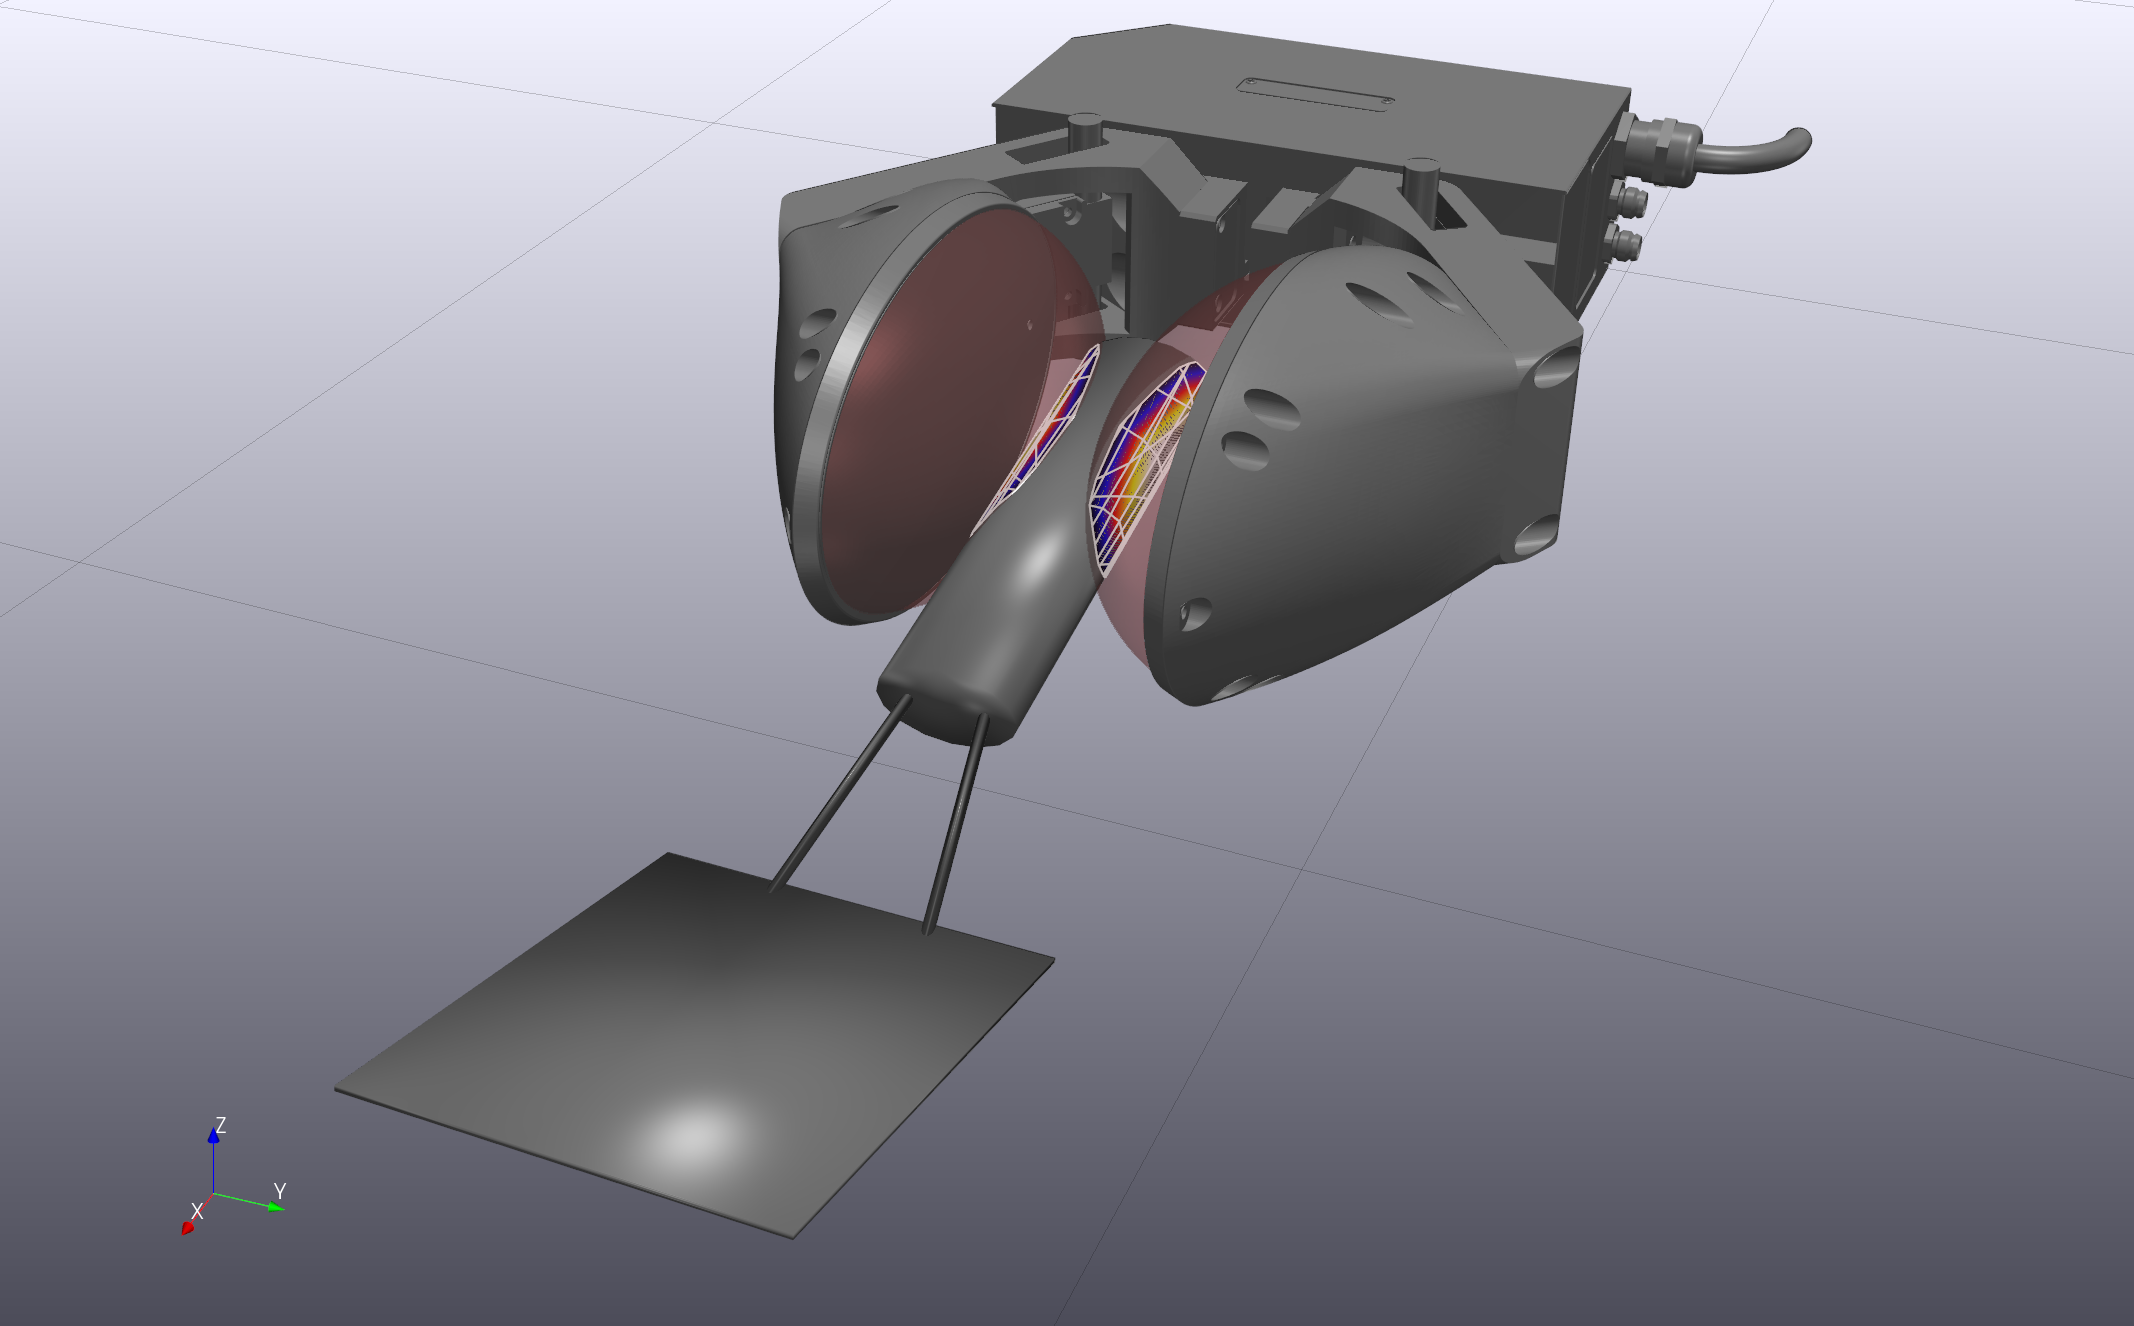
\includegraphics[width=0.8\columnwidth]{figures/slip_control/slip_control_single_frame.png}
	\caption{\label{fig:slip_control_frame} 
	Highly compliant \emph{Soft-bubble} gripper \cite{bib:kuppuswamy2020soft}
	holding a spatula. Unlike traditional point contact approaches, the
	hydroelastic contact model provides rich contact information and captures
	area-dependent phenomena such as the net-torque to hold the spatula. Contact
	patches are colored by contact pressure.}
\end{figure}

\begin{figure}[!h]
	\centering
    %trim={<left> <lower> <right> <upper>}
    \adjincludegraphics[width=0.49\columnwidth,trim={0 0 {0.05\width} 0},clip]{figures/slip_control/controller_force.png}
    \adjincludegraphics[width=0.49\columnwidth,trim={0 0 {0.05\width} 0},clip]{figures/slip_control/spatula_pitch.png}
	\caption{\label{fig:slip_control_history} 
	Grip force command (left) and spatula pitch angle (right) as a function of
	time.}
\end{figure}

We compare the performance of SAP against both Gurobi and Geodesic IPM, see
Section \ref{sec:about_solvers}. For SAP we use a relative tolerance
$\varepsilon_r=10^{-3}$, see Section \ref{sec:stopping_criteria}. For Gurobi we
set its tolerance parameter \verb+BarQCPConvTol+ to $10^{-8}$. For Geodesic IPM,
we set its complementary slackness tolerance to $10^{-6}$; larger values lead to
failure for this task. SAP bounds the momentum error, exhibiting a maximum value
of of $9.99\times 10^{-2}\,\%$. Even with such a tight tolerance, Gurobi
exhibits $2.6\,\%$ maximum error. Geodesic IPM's errors are significantly
smaller, below $2\times 10^{-4}\,\%$. However its robustness is very sensitive
to the specified tolerance.

Even though SAP's solutions are significantly more accurate than those from
Gurobi, it performs 92 times faster than Gurobi. SAP is 20 times faster than
Geodesic IPM and significantly more robust to solver tolerances. In terms of
solver iterations, SAP only performs 0.62 iterations on average, showcasing how
effectively it warm-starts. Geodesic IPM performs 5.6 iterations per step on
average and Gurobi performs 10.1 iterations on average.
